\Chapter{Tervezés}

Ennek a szekciónak a célja bemutatni a kották tárolásának különböző módszereit. Mindemellett hangsúlyt fog kapni az RDF modell felhasználása, valamint annak különböző szerializációját megvizsgálva megtekinthető, hogy milyen módon lehet tárolni és ezáltal lehetővé tenni a lekérdezését egy-egy kottának. Lekérdezés alatt ebben az esetben azt kell érteni, hogy az adott kotta milyen jellemzőkkel rendelkezik. Példának okán lekérdezhető a kotta hangneme, az hogy milyen akkordok szerepelnek a kottában, és más egyéb olyan információ amit hasznosítani tud a felhasználó. Vagy közvetlenül, vagy pedig közvetetten egy program segítségével.

\Section{RDF használata}
Az esetünkben felhasznált adatok ábrázolására a következőképpen nézne ki az RDF modell. Az akkord reprezentálná a hármasok közül a témát, vagyis a subject-et, mivel azt kellene először definiálni. Az akkord, ami más néven hármas hangzat, alapvetően három hangból épül fel. Van a fő hang, ami tegyük fel, ha C-dúr akkordot akarunk modellezni, az a C hang lesz, erre épül a dúr esetében a nagy terc, ami az E hangot fogja adni, valamint a C hanghoz igazított kvint távolságra levő G hang. Tehát a C-dúr akkordot a C E és G hangokból lehet összeállítani, ezek egyben fokok is, amiket predikátumként fogunk jelölni, hogy melyik hang az akkord hanyadik foka. Ezt a következő ábrán lehet látni.
\par
\begin{figure}[h]
	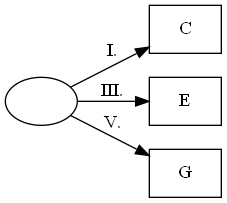
\includegraphics[scale=1]{images/img_src/rdf_graph.png}
	\caption{Szemantikus ábrázolás az RDF szerint.}
	\label{fig:graph1}
\end{figure}
\newpage
Az ábrán látható, hogy egy akkord meghatározásához 3 él vezet kifelé, ugye ezek jelzik, hogy melyik fokon található a C-dúr akkord hangjai (rendre I., III. és V. fok ) és az objektumok maguk a hangok, ahova az él mutat. Ebben az esetben meg is lenne oldva az akkordok ábrázolása RDF modell szerint, viszont a kottába való visszahelyezéskor a programnak szükséges tudnia azt is, hogy pontosan hova illessze vissza a megfelelő akkordot egy transzponálás esetében, mikor is a hangnem változik, és a kottába szereplő akkordok kicserélődnek. 
Ilyenkor szintén használva a gráf elméletét az akkord alatti szövegrész lesz az objektum, az él pedig elnevezve a pozíció lesz. Ugyanis a kottában szereplő szöveg nem változik ugye csak az akkordok, ha bármilyen művelet kerül végrehajtásra. Viszont, ha változik a szöveg, abban az esetben a pozíció is tud változni a szövegnek megfelelően. Többféle probléma merülhet fel, abban az esetben, ha statikusan akarom használni a doboz-t amit az akkordhoz kivág a program a szöveggel együtt, akkor annak a méretét egy kalkulált értékből kell kapnia, ami illeszkedik a megfelelő felbontáshoz, mert ahogy a felbontás különbözik az egyes kották képeinél, úgy változik a doboz mérete is arányosan.
\newpage
\Section{Kotta tárolási példák}
\SubSection{Music XML}
\begin{xml}
<?xml version="1.0" encoding="UTF-8"?>
<!DOCTYPE score-partwise PUBLIC "-//Recordare//DTD MusicXML 1.1 Partwise//EN" "http://www.musicxml.org/dtds/partwise.dtd">
<score-partwise>
   <part-list>
      <score-part id="P1">
         <part-name>Music</part-name>
      </score-part>
   </part-list>
   <part id="P1">
      <measure number="1">
         <attributes>
            <divisions>1</divisions>
            <key>
               <fifths>0</fifths>
            </key>
            <beats>4</beats>
            <beat-type>4</beat-type>
            <clef>
               <sign>G</sign>
               <line>2</line>
            </clef>
         </attributes>
         <note>
            <pitch>
               <step>C</step>
               <octave>4</octave>
            </pitch>
            <duration>4</duration>
            <type>whole</type>
         </note>
      </measure>
   </part>
</score-partwise>
\end{xml}

Ez a MusicXML egyik példája, a kotta tárolására. A mintaadathalmaz, tehát a kották, másképpen épülnek fel, nincsenek vonalak, vagy hangjegyek, ez egy ún. akkordos kotta, ami a következőképpen néz ki

\cite{enwiki:1065665260}
A MusicXML Michael Good találmánya és a Recordare LLC alatt történt a fejlesztése, majd 2011-ben a MakeMusic folytatta, aztán pedig 2015 óta a W3C Music Notation Community Group. Az első verziója 2004 januárjában jelent meg, később kapott olyan fejlesztéseket, amik a formázást támogatják jobban, ahogy a 2.0 verzióban már általános tömörített formátum is elérhető volt. Ebben a verzióban került bevezetésre az XSD használata, mivel eddig DTD-vel voltak definiálva.

\newpage
\SubSection{Saját kottatárolási módszer XML-ben}
\begin{figure}[h]
	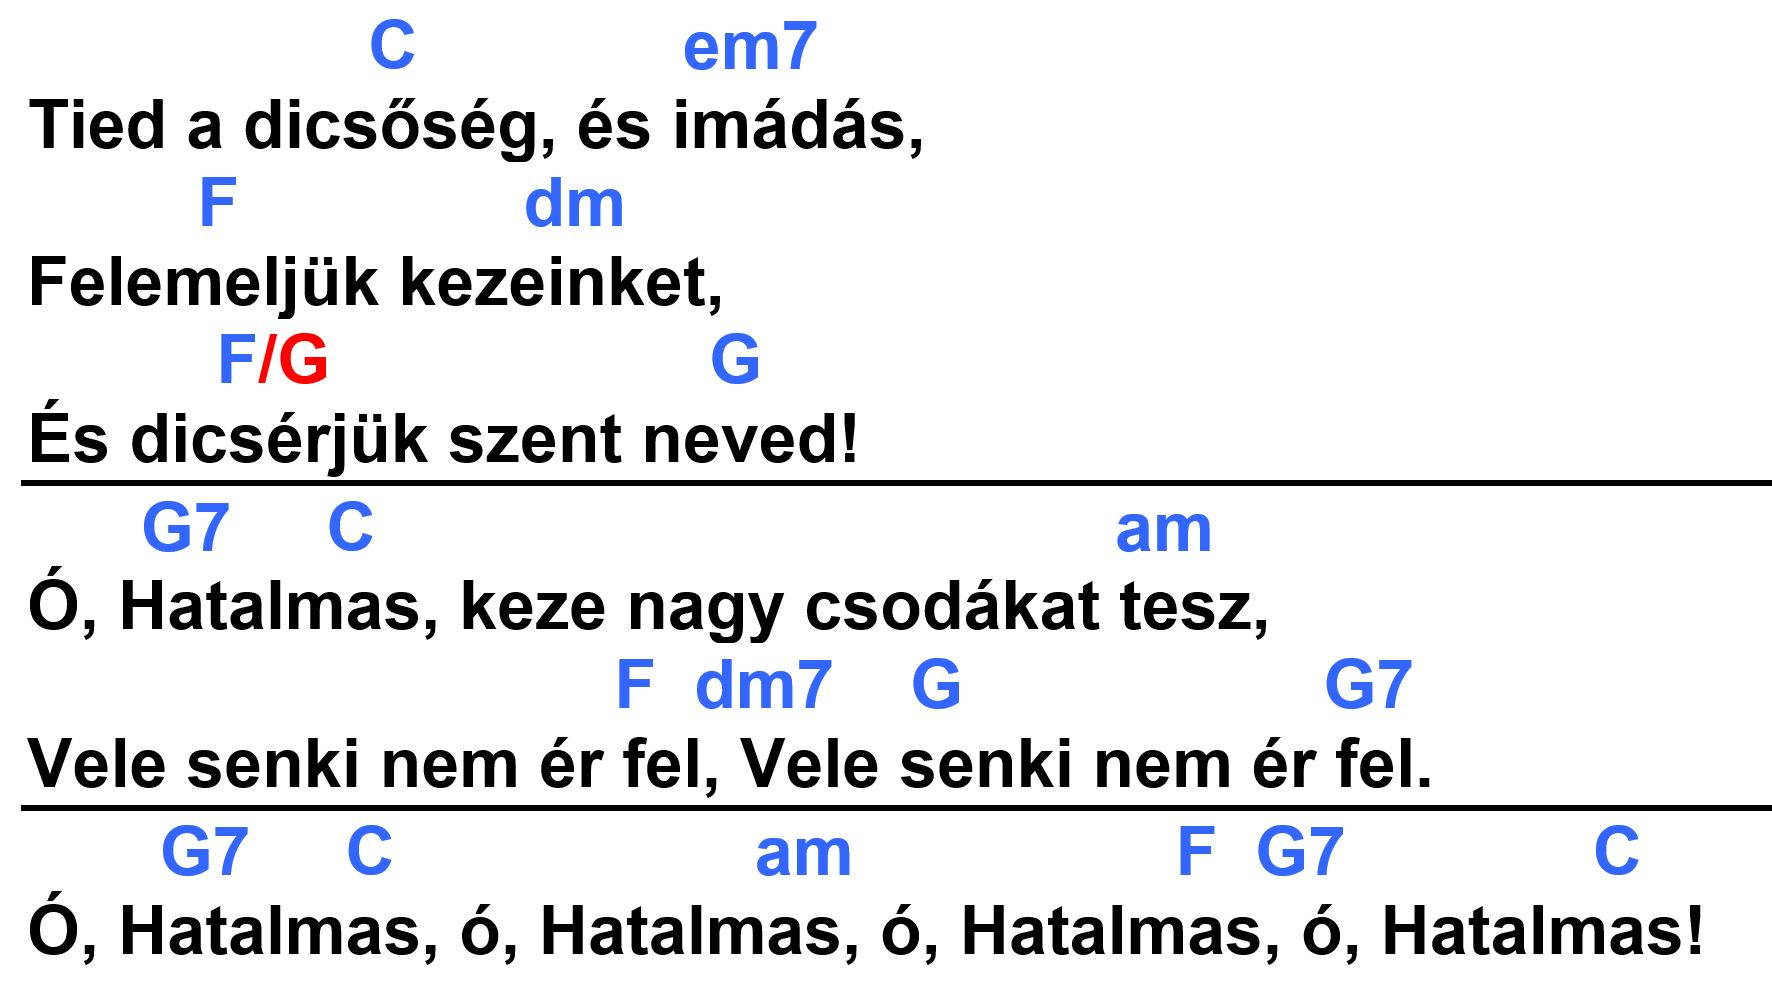
\includegraphics[scale=0.3]{images/samples/Tied_a_dicsoseg.jpg}
	\caption{A példa kotta.}
	\label{fig:song1}
\end{figure}

Ezt a példakottát használva, ha tárolni szeretnénk xml-be, az akkordokat, valamint a szöveget és azt, hogy az akkord az mely szövegrész felett helyezkedik el, mint az akkord pozíciója, akkor az egy ilyen xml-t eredményezne:

\begin{xml}
<?xml version="1.0" encoding="UTF-8"?>
<sheet>
   <key>
      <note>C</note>
      <chord>major</chord>
   </key>
   <segment id="1">
      <note>C</note>
      <text>Tied a dicsőség,</text>
      <position>őség</position>
   </segment>
   <segment id="2">
      <note>em7</note>
      <text>és imádás,\n</text>
      <position>im</position>
   </segment>
   ...
   <segment id="19">
      <note>C</note>
      <text>mas!</text>
      <position>mas</position>
   </segment>
</sheet>
\end{xml}

Ennek a kottának a doboz-illesztés szerint, amiről később szó lesz, 19 szegmense van. Így egy sémával bemutatva látható, hogy az xml lényegi része hogyan épülne fel.

\begin{xml}
<xs:schema attributeFormDefault="unqualified" elementFormDefault="qualified" xmlns:xs="http://www.w3.org/2001/XMLSchema">
  <xs:element name="sheet">
    <xs:complexType>
      <xs:sequence>
        <xs:element name="key">
          <xs:complexType>
            <xs:sequence>
              <xs:element type="xs:string" name="note"/>
              <xs:element type="xs:string" name="chord"/>
            </xs:sequence>
          </xs:complexType>
        </xs:element>
        <xs:element name="segment">
          <xs:complexType>
            <xs:sequence>
              <xs:element type="xs:string" name="note"/>
              <xs:element type="xs:string" name="text"/>
              <xs:element type="xs:string" name="position"/>
            </xs:sequence>
            <xs:attribute type="xs:byte" name="id"/>
          </xs:complexType>
        </xs:element>
      </xs:sequence>
    </xs:complexType>
  </xs:element>
</xs:schema>
\end{xml}

Szegmensekre van bontva az adott akkord és a hozzátartozó szöveg. Minden szegmens kap egy id-t ami a sortöréshez szükséges az első verzió szerint. A szegmensen belül a note tárolja az akkordot, a text a blokkhoz tartozó szöveget, a position pedig tárolja az akkord elhelyezkedését a szöveg felett. Python-ba ehhez készült egy szemléltető program, ami ezt az xml-t jeleníti meg egyenlőre konzolon.

\Section{XML feldolgozása}
\SubSection{Megfigyelések}
A jelen példában 3 részre van bontva a kotta, szöveg, akkord, pozíció. Ahhoz, hogy ebből tudjon  működni a konzolra kiiratás a megfelelő pozíciókkal, az indexelést tettem lista adatstruktúrába, hogy meglegyen mindegyik akkordnak a megfelelő pozíciója. Kétfajta adat kerül tárolásra, az egyik mindenképpen az, hogy az xml-ben megadott string alapján melyik indexű karakternél található a szegmens szövegében a string maga, mert az jelöli az akkord helyét. A másik pedig maga a string ami kiadja a kotta véglegesítését, a konkatenált akkord, - és szóközszámmal, valamint a kotta szövegével.

Az első elakadást az egy sorba történő többszöri előfodulású szöveg okozta, amit úgy oldottam meg, hogy ha már egyszer megtalálható a sorban az adott substring, akkor azt megszámolja hányszor fordul elő, annyiszor kihagyja azt és a következőt vegye számításba az indexelésnél. Ehhez tartozik a számláló, ami olyan értéket kap, amennyi előfordulása van a substringnek az addig befűzött sorba.

A beolvasás célja egyenlőre csak az, hogy a kotta kikerüljön a konzolra, lényegében, ha transzponálási műveletet akarunk végrehajtani a kottán, akkor ennél részletesebben szükséges megadni az akkordot. Ugye, ahogy fentebb is írtam, az akkord hármashangzatba(vagy négyeshangzat, a jelölésektől függően) gondolva alapjáraton az első a harmadik és az ötödik fokból áll, amikor dúrról beszélünk. Ehhez már szükséges, akkor az, hogy az xml létrehozásakor külön legyen választva a mol és a dúr is. Egységesen meg van oldva ez az összes kottára nézve, ami mol akkordokat jellemzik, azok a következők:
\begin{itemize}
	\item[--]az akkord kisbetűvel van
	\item[--]az akkord kisbetűvel van és mellette egy kis m betű áll (pl.: am egy a-molt jelöl)\linebreak
\end{itemize}
Ami pedig a dúr akkordokat jellemzik:
\begin{itemize}
	\item[--]az akkord nagybetűvel van
\end{itemize}

Ezeket amikor képes megkülönböztetni a program, akkor ennek megfelelően fogja tudni lementeni a note mellé azt a property-t ami jelöli, hogy az akkord az mol vagy dúr. Legyen a neve mondjuk tone. Ebből kiindulva így nézne ki az egyik szegmens:
\begin{xml}
<segment id="12">
   <chord>
      <note>G</note>
      <tone>major</tone>
   </chord>
   <text>senki nem ér</text>
   <position>se</position>
</segment>
\end{xml}

Miután meg lehet különböztetni a mol-t a dúrtól, ezután mivel akkordról beszélünk, ami legtöbb esetben hármas hangzat, azt is fel kell osztani. Az akkord a hang diatonikus I. III. és V. fokából épül fel, valahogy így nézne ki, ha letárolnánk xml adatstruktúrába csak egy szegmensét:
\begin{xml}
<segment id="12">
   <chord>
      <note>G</note>
      <measures>
         <I>G</I>
         <III>H</III>
         <V>D</V>
      </measures>
      <tone>major</tone>
   </chord>
   <text>senki nem ér</text>
   <position>se</position>
</segment>
\end{xml}

\Section{RDF szerializációk}

\SubSection{RDFa}

\cite{rdfa_with_example}
Az RDFa egy olyan szerializáció, ami a legjobban egy html stílusú felépítésre hasonlít. A struktúra, valamint a hierarchia azonosítható, mindemellett biztosítja a prefix lehetőséget is és nagyon könnyen lehetővé teszi a bővítést is. A következő példában figyelhető ez meg:

\begin{xml}
<div vocab="http://xmlns.com/foaf/0.1/" resource="#12" typeof="Segment">
    <a href="chord">G</a>
    <span property="text">senki nem ér</span>
    <span property="position">se</span>
    <div property="chord" typeof="Chord">
        <span property="note">G</span>
        <span property="I.">G</span>
        <span property="III.">H</span>
        <span property="V.">D</span>
        <span property="tone">major</span>
    </div>
</div>
\end{xml}

Egy fő div tag (ejtsd: teg) adja meg a kiinduló csomópontot, ez például az xml-ben volt a <segment>...</segment> tag. Ez alá hierarchikusan felépülnek szinte irányított gráfként a további csomópontok, amik lehetnek egyszerű tulajdonságok, vagy referenciák egy másik objektumra.

\begin{figure}[h]
	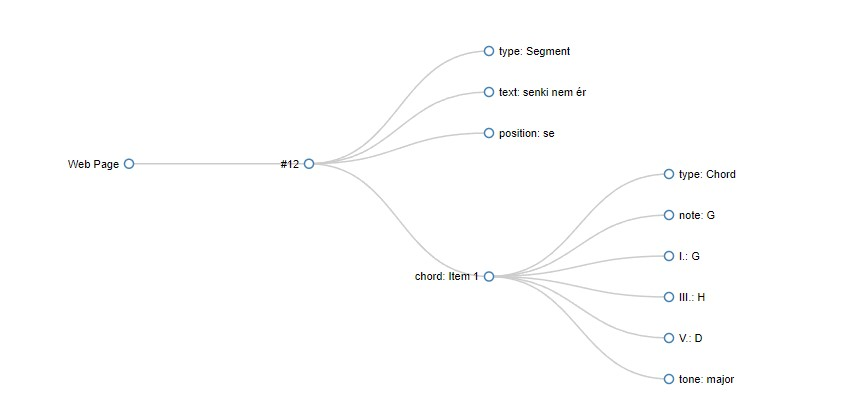
\includegraphics[scale=0.8]{images/misc/RDFa_serialization_example.jpg}
	\caption{Az RDFa szerializáció ábrázolása.}
	\label{fig:rdfa}
\end{figure}


\SubSection{Turtle felhasználása}
\begin{itemize}
\item A Turtle-ről néhány szó(https://www.w3.org/TR/turtle/)
\item Hogyan használható a jelen esetben
\item Esetek leírása Turtle-el
\end{itemize}

A Turtle egy olyan leíró nyelv, mely a szöveges reprezentációját mutatja be az RDF gráfos megjelenítésének.
\begin{xml}
<http://sheet_example.com/segment> <http://sheet_example.com/segment/id> "12".
<http://sheet_example.com/segment> <http://sheet_example.com/segment/chord> <http://sheet_example.com/segment/#chord>.
<http://sheet_example.com/segment> <http://sheet_example.com/segment/text> "senki nem ér".
<http://sheet_example.com/segment> <http://sheet_example.com/segment/position> "se".
<http://sheet_example.com/segment/12/#chord> <http://sheet_example.com/segment/12/#chord/note> "G".
<http://sheet_example.com/segment/12/#chord> <http://sheet_example.com/segment/12/#chord/I.> "G".
<http://sheet_example.com/segment/12/#chord> <http://sheet_example.com/segment/12/#chord/III.> "H".
<http://sheet_example.com/segment/12/#chord> <http://sheet_example.com/segment/12/#chord/V.> "D".
<http://sheet_example.com/segment/12/#chord> <http://sheet_example.com/segment/12/#chord/tone> "major".
\end{xml}

A Turtle lehetőséget ad a base révén arra, hogy egy, a jelenleginél értelmezhetőbb reprezentációt lehessen létrehozni, mégpedig a következőképpen:

\begin{xml}
@base <http://sheet_example.com/>.

<segment> <segment/id> "12".
<segment> <segment/chord> <segment/#chord>.
<segment> <segment/text> "senki nem ér".
<segment> <segment/position> "se".
<segment/12/#chord> <segment/12/#chord/note> "G".
<segment/12/#chord> <segment/12/#chord/I.> "G".
<segment/12/#chord> <segment/12/#chord/III.> "H".
<segment/12/#chord> <segment/12/#chord/V.> "D".
<segment/12/#chord> <segment/12/#chord/tone> "major".
\end{xml}

Látható, hogy a @base-ben megadott érték többször szerepel az elsőnek megadott példában, így megoldható az, hogy leegyszerűsítve egy @base annotációval olvashatóbb legyen a szerializáció. Emellett fontos megemlíteni azt, hogy ez a szerializáció akkor megy át a validáción, ha .-al zárul le egy-egy hármas.

\SubSection{RDF/XML}
A már létrehozott szimpla xml-ből látható, hogy mit is jelent az RDF/XML. Egy ugyanolyan xml kiterjesztésű fájlról beszélünk, viszont egyértelműen a felhasználása arra irányul, hogy egy bármely rdf könyvtárral használható, lekérdezhető legyen. Ebben segítenek a névterek. Ezek a névterek úgy jönnek létre, ahogy az irányított gráfokban látható név nélküli csomópontok is. Itt úgymond ezek a "név nélküli" csomópontok nevet kapnak a névterezés által.
Így néz ki egy részlete:

\begin{xml}
	<?xml version="1.1" encoding="UTF-8" standalone="no"?>
	<rdf:RDF 
			xmlns:rdf="http://www.w3.org/1999/02/22-rdf-syntax-ns#"
			xmlns:key="http://sheet_example.com/key/"
			xmlns:segment="http://sheet_example.com/segment/"
			key:chord="http://sheet_example.com/key/chord/"
			segment:chord="http://sheet_example.com/segment/chord/">
	
	    
	        <rdf:key>
	            <key:chord>C</key:chord>
	            <key:tone>major</key:tone>
	        </rdf:key>
	        <rdf:segment id="1">
	            <segment:note>C</segment:note>
	            <segment:text>Tied a dicsőség, </segment:text>
	            <segment:position>őség</segment:position>
	        </rdf:segment>
	        <rdf:segment id="2">
	            <segment:note>em7</segment:note>
	            <segment:text>és imádás,\n</segment:text>
	            <segment:position>im</segment:position>
	        </rdf:segment>
	        ...
	        <rdf:segment id="19">
	            <segment:note>C</segment:note>
	            <segment:text>mas!</segment:text>
	            <segment:position>mas</segment:position>
	        </rdf:segment>
	
	
	</rdf:RDF>
\end{xml}

A példaként szolgáló programomban a lekérdezés bemutatásához azért ezt a szerializációt használtam, mert ez a legelemibb tárolásra képes. A Turtle és az RDFa az sokkal inkább a megjelenítéskor játszhat szerepet, legfőképp az RDFa a html struktúrája miatt. A jelenlegi szerializációban, az első verziót használtam, lényegében csak a pozíció, a szöveg és az akkord egyedülálló letárolása van meg.


\Section{Szemantikus ábrázolás RDF-el}



\begin{figure}[h]
	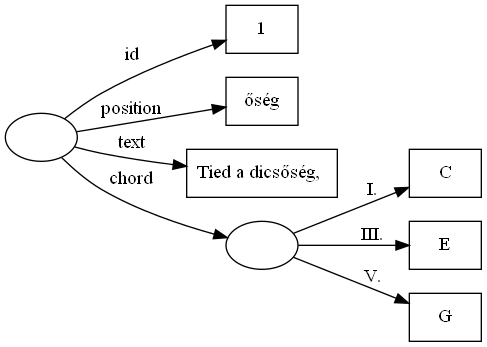
\includegraphics[scale=0.5]{images/img_src/rdf_graph_2.png}
	\caption{Konkrét szemantikai ábrázolása a dal egy szegmensének.}
	\label{fig:graph2}
\end{figure}
\par
A \ref{fig:graph2}-es ábrán látható, hogy az adott példa kottánkban hogy nézne ki egy szegmens. A szegmens most jelen esetben az akkord és az ahhoz tartozó szöveg leírása. A jelenlegi kottához 19 db ilyen szegmens tartozik, indexelve az akkord alapján, tehát 19 akkord van a dalban. A kiinduló elemből az első elágazás az id-hoz vezet, nagyon egyszerűen, ez csak az azonosító száma a dalban szereplő szegmensnek. Ezek alapján például úgy csináltam meg a programot, hogy egy tömb adatstruktúrába adtam meg neki, hogy melyik szegmensnél történik a sortörés, és azoknál a szegmenseknél belefut a program egy plusz ágba, ahol sortörés és a változók újrainicializálása történik. Onnantól következik a pozíció, ami azt a szövegrészt tárolja a szegmensből, ami egyedien azonosítja, hogy az akkord pontosan hol helyezkedik el a szegmensben, egyenlőre ez egy változó hosszúságú string, de érdemes meghatározni, hogy 3 esetleg 4 hosszúsággal történjen ugye a kiolvasás a következetesség szempontjából. 
\par 
A következő elágazás a szövegre mutat, tehát ami konkrétan benne lesz majd a végkifejletbe, ebből származik a pozíció, amiről fentebb szó volt már. Ezután következik az akkord, ami a jelenlegi ábrázolásba úgy néz ki, hogy a szegmens akkordja az egy C, viszont a tonika az külön meghatározandó, vagyis, hogy dúr vagy mol az adott akkord. Az akkordból 3 predikátum mutat objektumokra és ez az amiből felépül egy akkord. Az első fok mutat az alaphangra, a harmadik a tercére az alaphangnak, amiből megállapítható, hogy mol vagy dúr az akkord, mert ha mol, akkor az alaphangra épített kis tercről van szó ami jelen esetben nem így van, hiszen a C - re épített nagy terc az E hang, tehát ez az akkord dúr. És a harmadik objektum az ötödik fok, tehát az alaphang, vagyis a C hang tiszta kvintre levő távolsága, azaz a G hang.\newpage

\begin{figure}[h]
	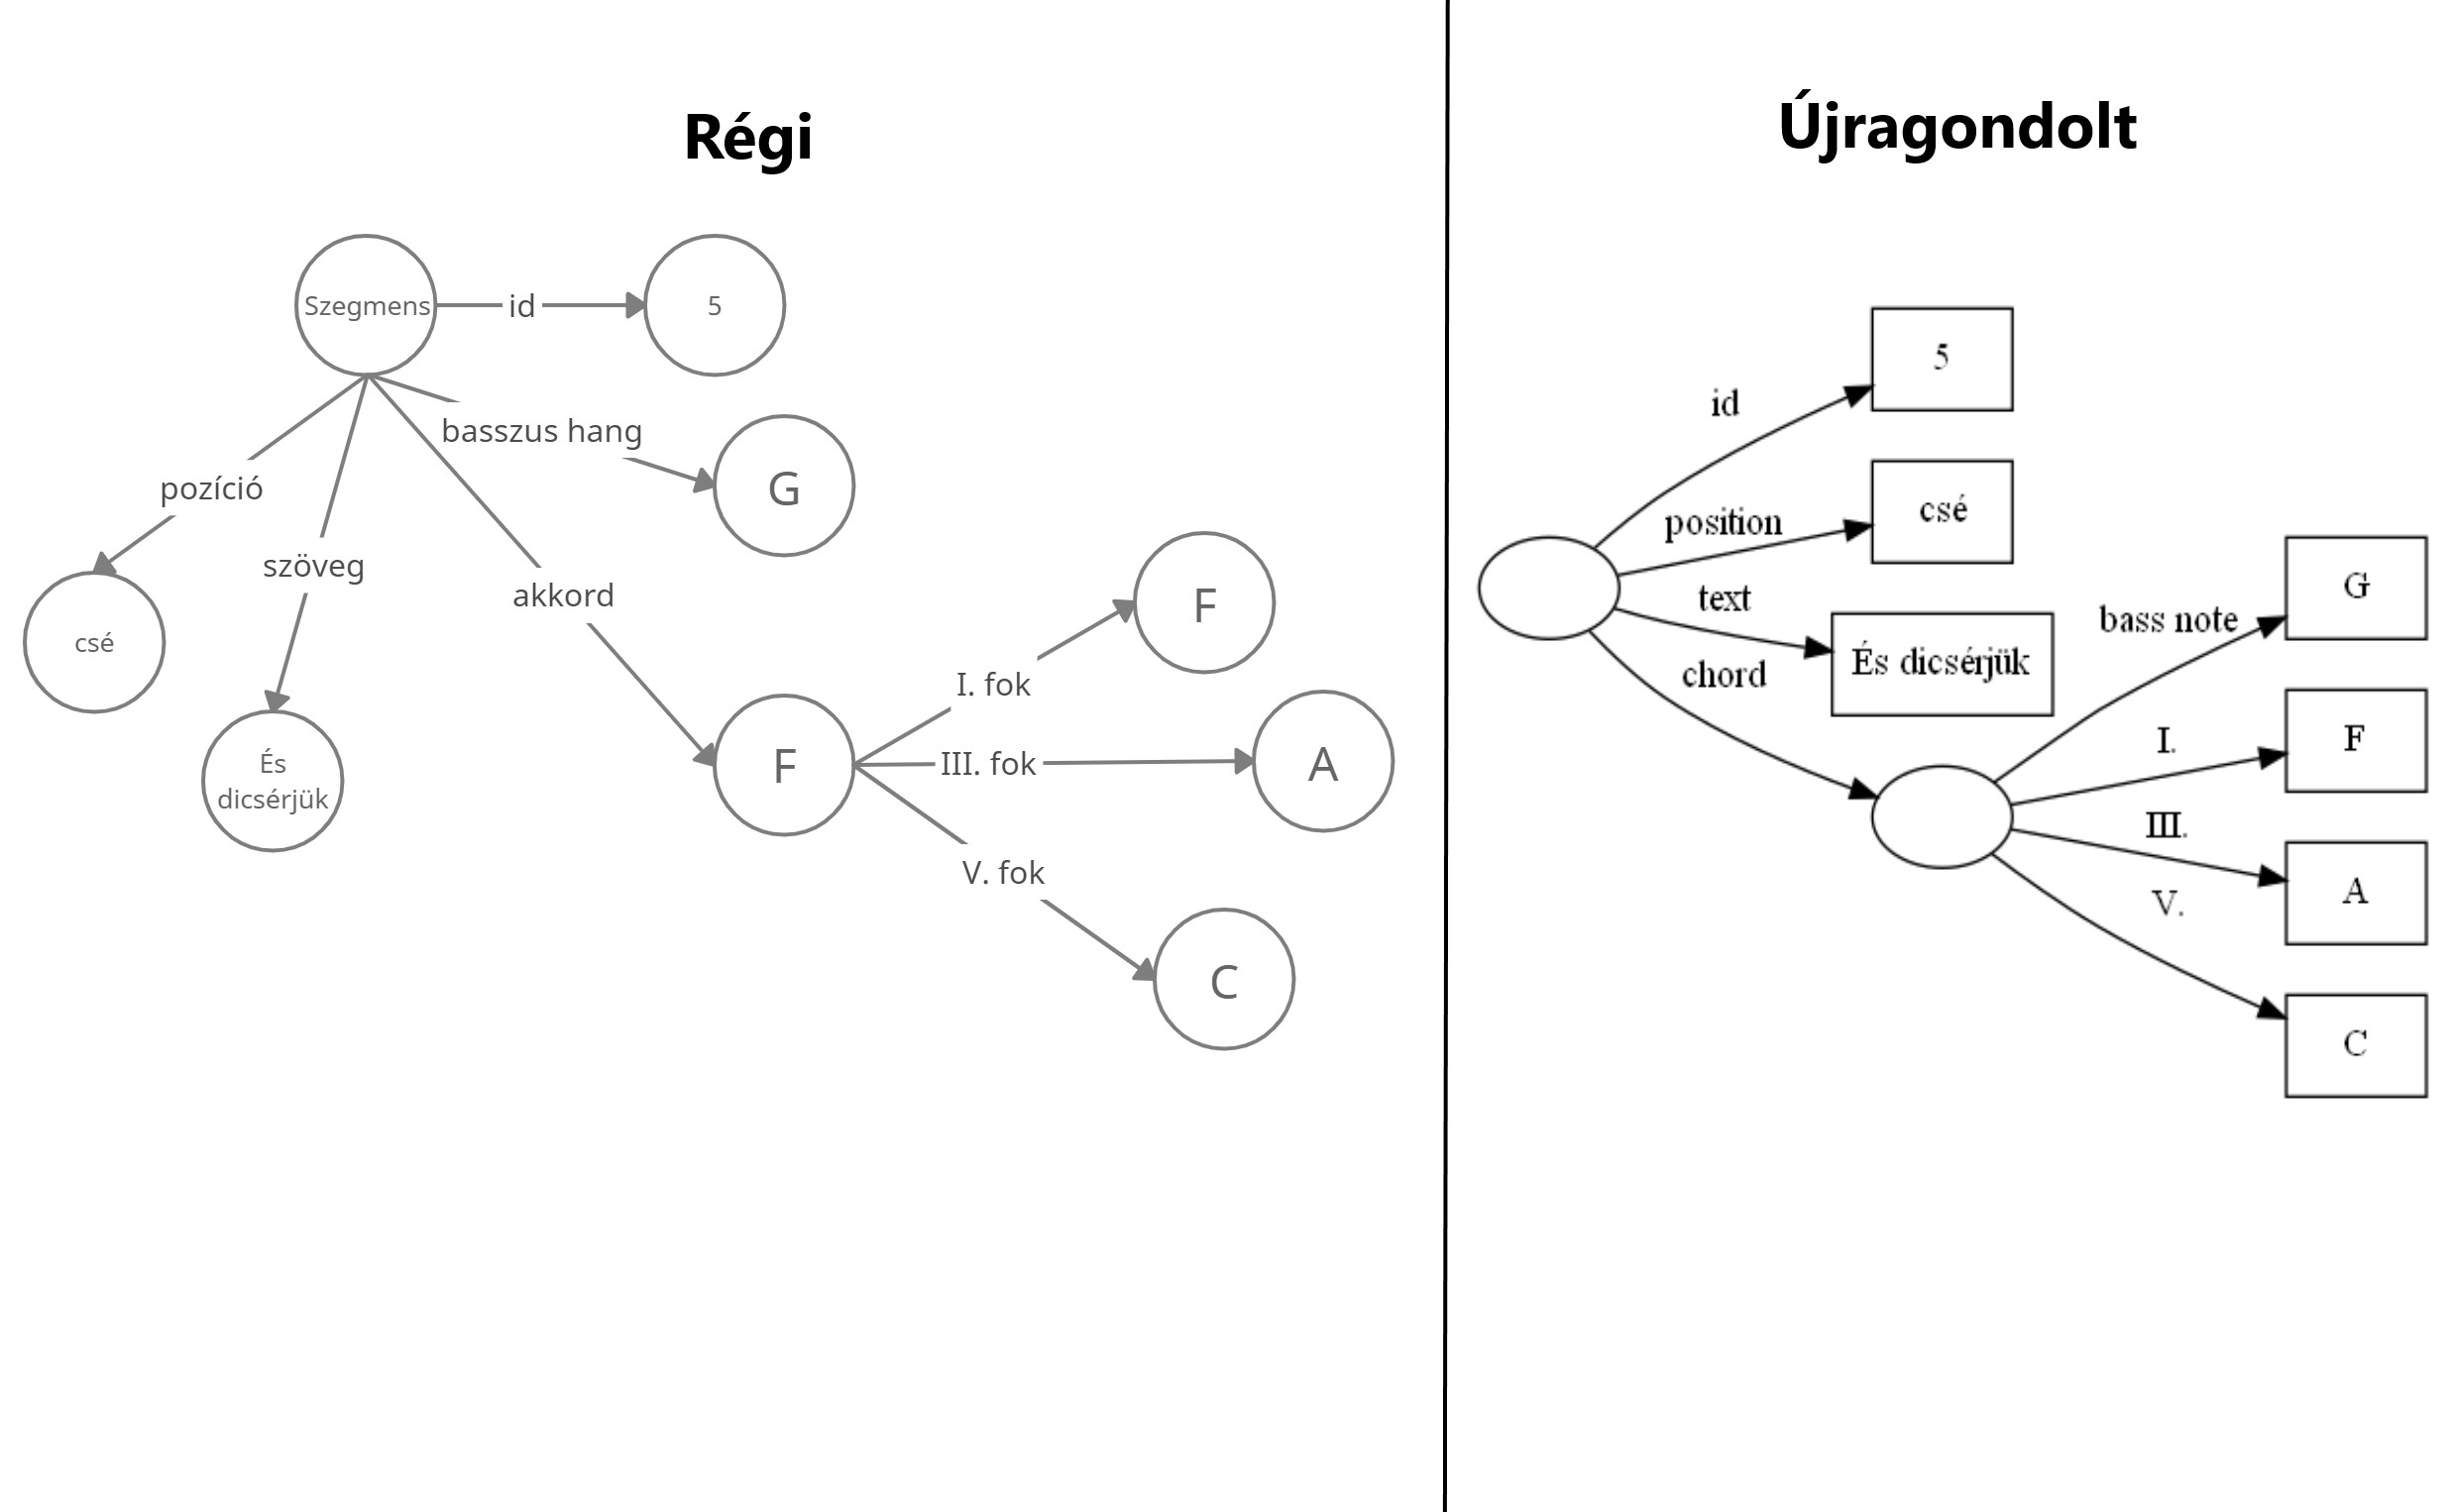
\includegraphics[scale=0.22]{images/misc/comparison_graph_3.jpg}
	\caption{Egy másik szegmens leírása}
	\label{fig:graph3}
\end{figure}

Ebben a szegmensben figyelhető meg, hogy az akkordhoz tartozik egy per basszus hang, ami most a G hang. Ez a kottában a következőképpen jelenik meg: \texttt{F/G} ekkor, az F kék színnel, míg a G az piros színnel van jelölve. Ahogy látható a \ref{fig:graph3}-ös ábrán is, a régi megoldásban nem az akkordhoz tartozik a basszus hang, hanem magához a szegmenshez, tehát nem az akkordot írja le ez az objektum, hanem a szegmenst. Habár nem mindegyik akkordnál jelez a kotta per basszus hangot, és azért tűnt egyszerűbbnek a szemantikus ábrázolása a basszus hangnak, mégis helytelen volt ebben az állapotában, ezért igényelt újragondolást. Az újragondolt ábrázolásban, már az akkordot írja le a basszus hang, hiszen az szintén az akkord, mint hármas hangzatnak a predikátuma. Alapesetben, mikor nincs a kottában jelezve a per basszus, akkor az akkord első fokát (I.) vesszük alapértelmezettnek. \par
A basszus hang, amikor nincs jelölve, akkor az akkord alaphangja, általában az akkord diatonikus harmadik foka szokott lenni még a basszus hang, de ez egy teljesen változó hang ilyen szempontból. Abban az esetben, ha kellene változó szeparáló elem, akkor külön lenne szedve valószínűleg, hogy a szegmenshez tartozna egy sima basszus, annak lenne a hangja a G és a szeparáló elem lenne mondjuk a \textbackslash. De mivel egységes a szeparáló elem a basszus hangnál ezért ez nem is szükséges, egyébként a szeparáló elem: \texttt{/}.
\par
Ha ugyanazt a szegmenst nézzük, akkor behozható a következő eset, amikor ugyanis meg kellene határozni, hogy az akkord az mol vagy dúr tonikájú. Ez mindenképpen egy olyan jelölő, ami az akkordot írja le, tehát azon belül szerepelne ez, és ahogy lesz szó arról, hogy miként épül fel egy hármas, így látni fogjuk majd, hogy a bemeneti oldalról miként lesz megkülönböztethető.
\par
\newpage

\begin{figure}[h]
	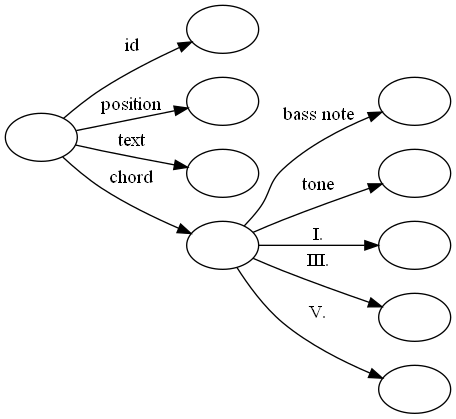
\includegraphics[scale=0.5]{images/img_src/rdf_graph_4.png}
	\caption{Bővített leírása a szegmensnek}
	\label{fig:graph4}
\end{figure}
A tonika az egy olyan predikátum, amivel leírható, hogy a hármashangzat, tehát az akkord az mol hangzású, avagy dúr hangzású, ami a kimenetnél abban hordozza a jelentőséget, hogy szemantikusan kisbetűvel -,és m-el végződve legyen megjelenítve az akkord vagy egyszerűen nagybetűvel. A \ref{fig:graph4}-os ábra mutatja, hogy az akkord a tonika predikátummal kiegészítve már 4 objektummal van leírva.
\par
Abban az esetben, hogy ha ismerjük az akkord hangjait, ugyanis abból már megállapítható az akkord, ha ismerjük az első fokot, akkor a három hang vagyis a három fok ismeretében egyértelműen megállapítható a tonika is. Egy dúr akkord ugye az első foktól számított nagy terc, majd kis tercből épül fel. Ezzel szemben egy moll tonikájú akkord az első foktól számított kis terc, majd nagy tercből épül fel. Így a három hangot ismerve rá lehet jönni arra, hogy dúr akkordról vagy moll akkordról van szó.
\par
Amikor meg tudjuk határozni a tonikát, akkor jöhet a következő lépés, ami arról szólna, hogy mi történik akkor, amikor a bemeneti kottában előfordul olyan, hogy transzponált akkord, és mi is ez valójában? Tömören, egy dal mindig egy meghatározott hangnemben van.
\newpage
\begin{figure}[h]
	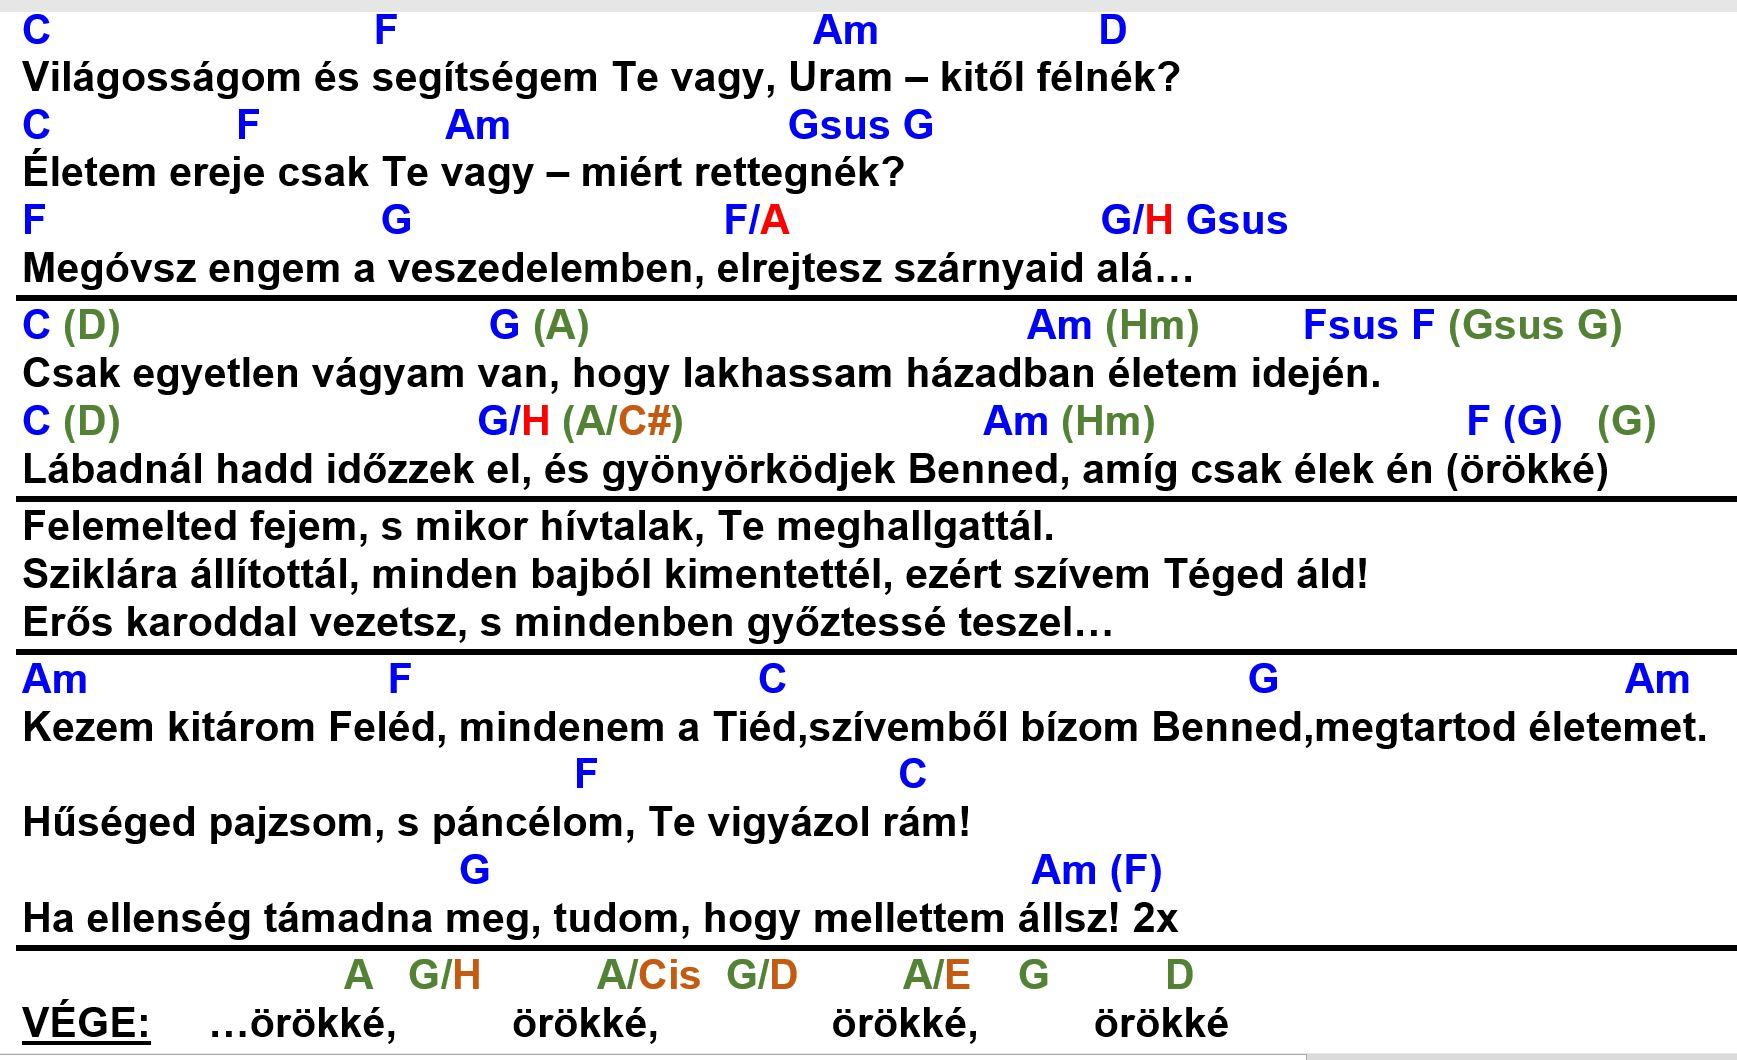
\includegraphics[scale=0.3]{images/samples/27_zsoltar.jpg}
	\caption{Példa kotta a transzponálás leírására}
	\label{fig:song2}
\end{figure}
Ez a következő példakotta, ami abban különbözik, az eddigitől, hogy a zölddel, valamint narancssárgával jelölt akkordok is megjelennek, amik egyébként a transzponálást jelzik dal közben. Sűrűsödnek az akkordok, itt a doboz-kezelést úgy kellene megoldani, hogy több akkordot is egybefogni, például, ahol egy-két szóköz van közötte és azt egybe kezelni. A zárójeles szeparátor egyértelműen mutatná, hogy itt transzponált akkordról van szó, viszont az utolsó előtt sor fölött látható, hogy kékkel jelölt zárójeles akkord van. Az az ismétlést hivatott jelezni, így a szeparátor nem adja meg egyértelműen, hogy most az akkord az transzponált e. A transzponáltságot tehát mindenképp a szín fogja eldönteni.

A következő esetek merülhetnek fel ezzel a kottával kapcsolatban:
\begin{center}
	\begin{tabular}{ |p{7cm}|p{7cm}| }
		\hline
		Eset(ek) & Megoldás\\ 
		\hline
		\begin{itemize}
			\item[--] Sűrűsödött akkordok
			\item[--] Zsúfoltság
			\item[--] Pozíció szempontjából esélyes, hogy félreindexelés történik
			\item[--] A substringet nem is találná meg a program, és az lehet nem is létezne hozzá
		\end{itemize} & A doboz-kezelést át kell formázni úgy, hogy képes legyen több akkordot is egybesűríteni és ezáltal a pozíciót rendesen belőni, és emellett az egybesűrűsített akkordok egymástól levő távolságát is megtartani \\ 
		\hline
	\end{tabular}
\end{center}
\newpage
\begin{figure}[h]
	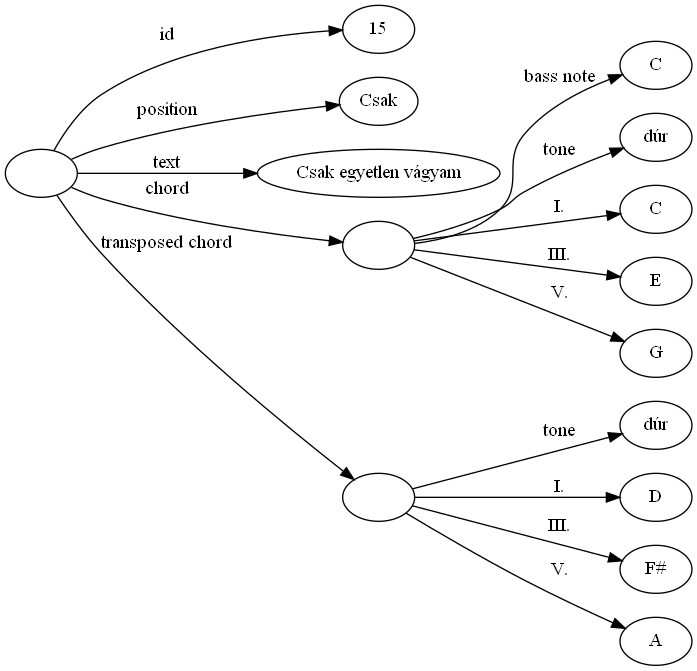
\includegraphics[scale=0.5]{images/img_src/rdf_graph_5.png}
	\caption{Szegmens leírása ahol transzponálás is van}
	\label{fig:graph5}
\end{figure}
Abban az esetben, hogyha van transzponált akkord a kottában, akkr azt egy másik akkordként lehet kezelni. Ez nem egy gyakori eset, tehát lehet először ahhoz kötni, hogy az nincsen, abban az esetben a 'transzponált' nevű predikátum a 'Nem' objektumra mutat. Így viszont ugyanúgy kezelendő mint egy akkord, van tonikája és legalább 3 foka, amiből felépül az akkord.
\newpage
\begin{figure}[h]
	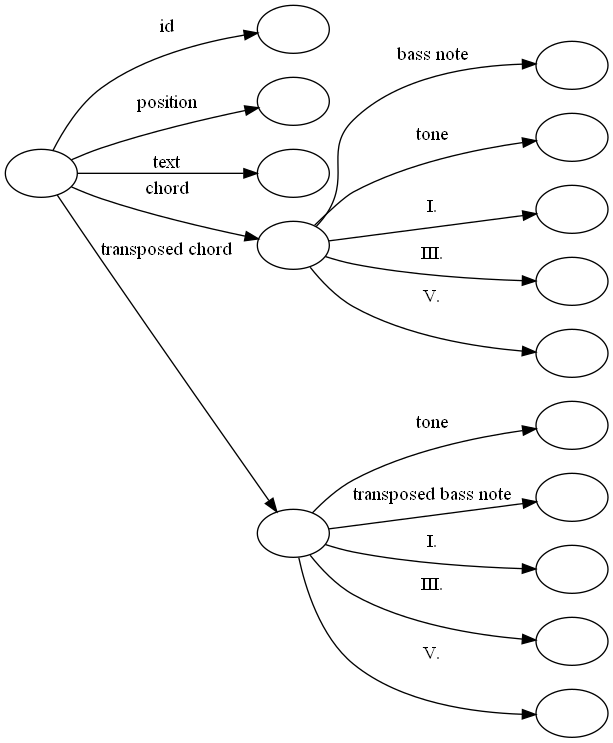
\includegraphics[scale=0.5]{images/img_src/rdf_graph_6.png}
	\caption{Szegmens leírása ahol a transzponálásban basszus hang van}
	\label{fig:graph6}
\end{figure}

A sima ábrázolásban látható, hogy a legbonyolultabb kotta szegmens az már elég szerteágazó irányított gráf lett. Itt amit érdemes megfigyelni, hogy az id, szöveg, pozíción kívül előfordulhatnak redundáns objektumok. Például a tonika a basszus hang predikátumok többször is előfordulhatnak, sőt, ha tonikáról beszélünk, akkor ott nem történhet olyan, hogy a szegmens akkordjának a tonikája különböző legyen, mint a transzponált akkord tonikája, tehát abban az esetben az az objektum biztosan többször is szerepelne az ábrán. Mindemellett az a vizsgálata a szegmensnek, hogy transzponált-e az egy egyszerű bool értékkel van leírva, ami ugyanúgy előfordulhat az ábrán más alanyhoz rendelve. Így a következő ábrán lehet látni, hogy az egyszerűsítés érdekében hogyan lehetne ezeket az ismétlődő objektumokat megszüntetni.

\begin{figure}[h]
	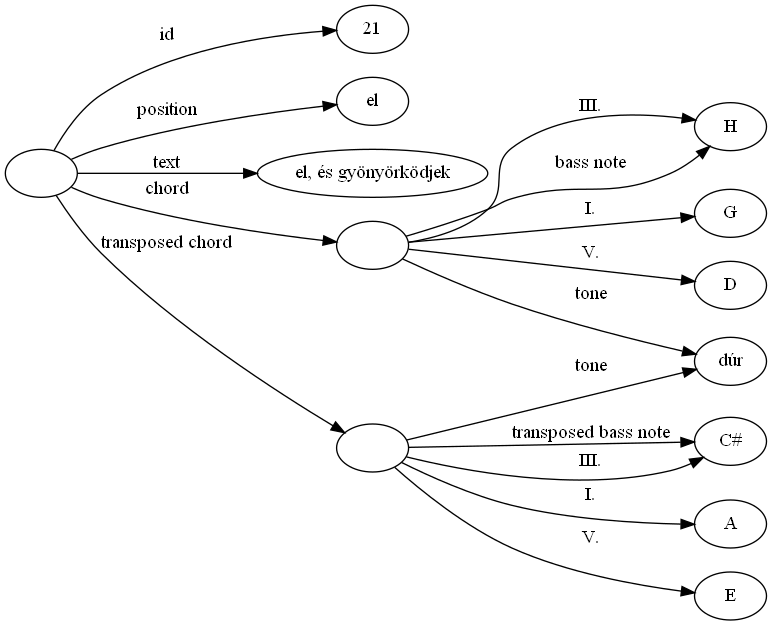
\includegraphics[scale=0.5]{images/img_src/rdf_graph_7.png}
	\caption{Szegmens redundancia mentes leírása}
	\label{fig:graph7}
\end{figure}
\newpage
Változtatások:
\begin{itemize}
	\item[--] Egyetlen objektum tartozhat más alanyokhoz
	\item[--] Az akkordokhoz tartozó fokok átnevezése
\end{itemize}

Ezen felül észrevehető az, hogy minden akkord, ami jelölve van, annak az első foka ugyanazt az értéket fogja kapni. Innen két irányba is mehetne az ábrázolás. Az első az lehetne, hogy akkor az akkord és a hang az külön jelentőséget képvisel, emiatt nem hivatkoztatható önmagába, tehát akkor a \ref{fig:graph7}-es ábra maradna. A másik viszont az, hogy a predikátum egy üres objektumra mutatna, és ezáltal létezne egy új predikátum ami az üresből elemből mutatna kifelé.

\Section{Adatfeldolgozás}
\SubSection{Kottaadatok tárolása}

Kiindulópontnak egy xml fájlt veszünk, ahol az egyszerű adatok kerülnek letárolásra, szegmentálva akkordok, szövegek és az akkordok pozíciói a szöveghez képest. Ehhez társul egy olyan program, ami betölti az xml fájlt, feldolgozza azt, hogy ezek az adatok elérhetővé váljanak ábrázolásra, valamint ezáltal lekérdezésre is. A programnak képesnek kell lennie arra, hogy az adott kotta adathalmazt elérje lekérdezések formájában.

\begin{figure}[h]
	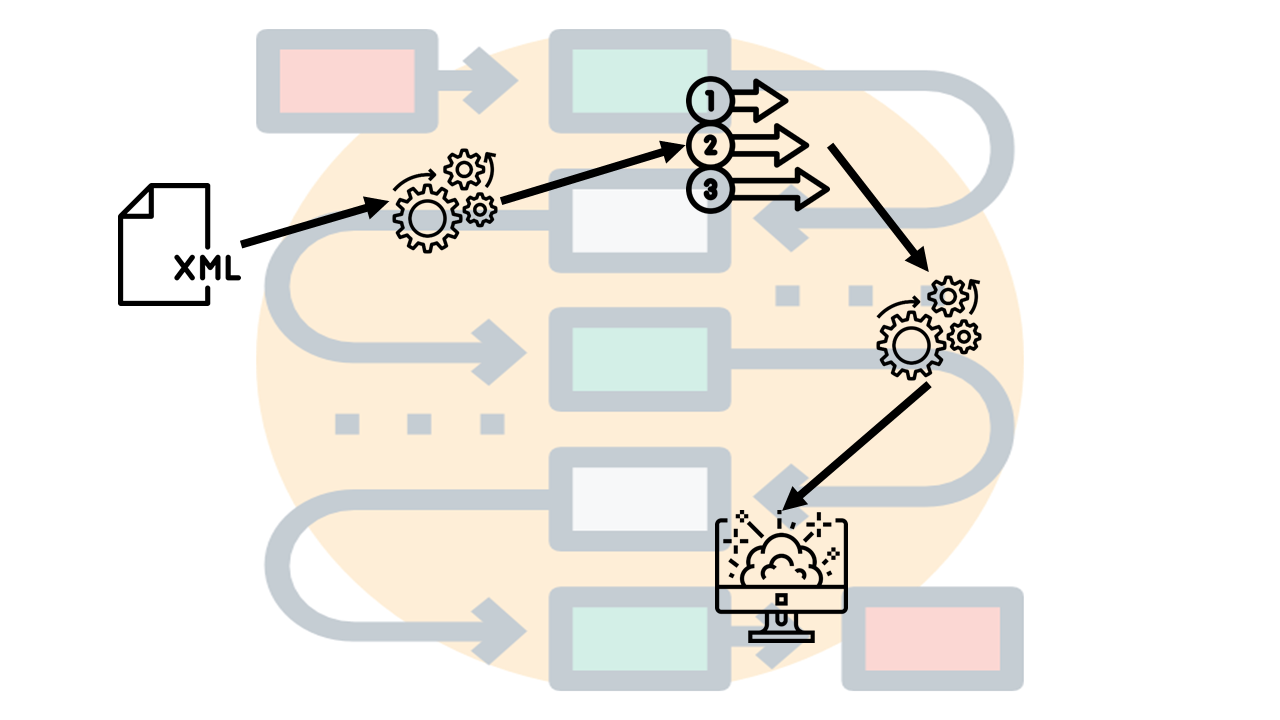
\includegraphics[scale=0.45]{images/presentation/data_flow.png}
	\caption{Adatáramlás és feldolgozás}
	\label{fig:flow1}
\end{figure}

\Section{Ábrázolás előnyei, hátrányai}
\SubSection{Irányított gráf ábrázolás}
\begin{center}
	\begin{tabular}{ |p{7cm}|p{7cm}| }
		\hline
		Előnyök & Hátrányok\\
		\hline
		Részletesen leírható bármilyen alany az ábrázolással & A gyökér, vagyis a kiinduló elem Szegmens-ként lett elnevezve, viszont mint elnevezés létezik csak, a gyökér elem hiánya \\ 
		\hline
		Az elnevezett élekkel pontosan megadható az, hogy mi jellemzi az alanyt & Az egy-egy kapcsolat miatt, nem lehet meghatározni ugyanazon predikátum alatt több tulajdonságot az alanyról\\
		\hline
	\end{tabular}
\end{center}

\begin{figure}[h]
	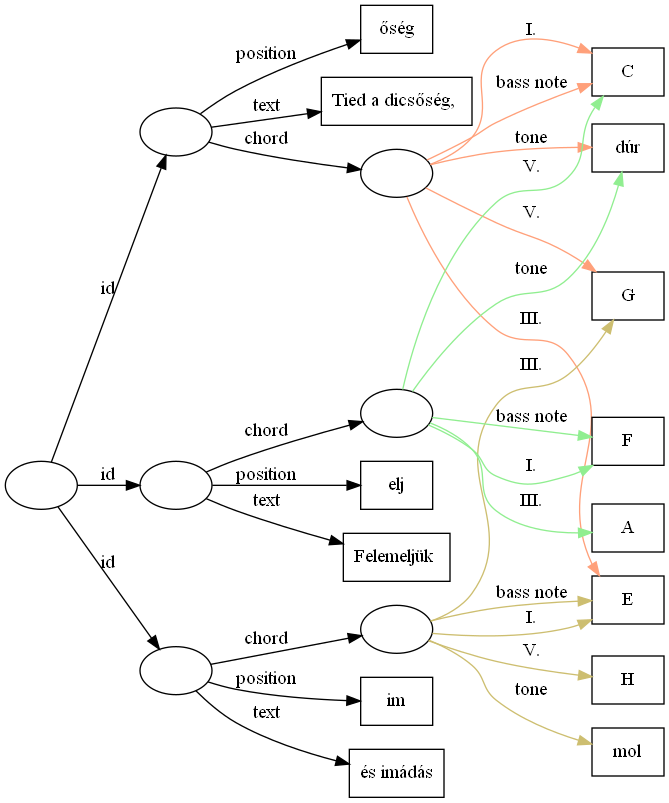
\includegraphics[scale=0.45]{images/img_src/representation_of_sheet.png}
	\caption{A kotta első három szegmense}
	\label{fig:repres1}
\end{figure}
\newpage
\SubSection{A \ref{fig:repres1}-es szemantikus ábra}
\begin{center}
	\begin{tabular}{ |p{7cm}|p{7cm}| }
		\hline
		Előnyök 
		& 
		Hátrányok
		\\
		\hline
		Az egyszerűsített ábrázolás redukálja a gráf túlságos szétterjedését 
		& 
		A jelenlegi kotta 19 szegmensből áll, ezt viszont így ábrázolni nem lehetne megfelelően 
		\\ 
		\hline
		Színezett predikátum-nyilak egyértelműsítik azt, hogy melyik objektumról van szó és az mely csomóponthoz tartozik pontosan
		& 
		Zavaró ellenben az, hogy a predikátum elnevezés melyik nyílhoz tartozhat pontosan. Ilyenkor érdemes leszögezni, hogy az ábrán milyen séma szerint van jelölve (jelen esetben a predikátum elnevézese mindig a nyil fölött lesz)
		\\ 
		\hline
		Az ábrán egyértelműen megkülönböztethető mindegyik szegmens, ez átláthatóvá teszi azt, hogy miként épül fel a kotta
		& 
		A sorrendiség nincs letárolva, ehhez szükséges lenne mindegyik szegmensnek beiktatni egy 'order' vagy egy 'rank' objektumot ami egyértelműen meghatározza, hogy az adott szegmens az melyik szegmens után jön netán az első e.
		\\ 
		\hline
	\end{tabular}
\end{center}

\begin{figure}[h]
	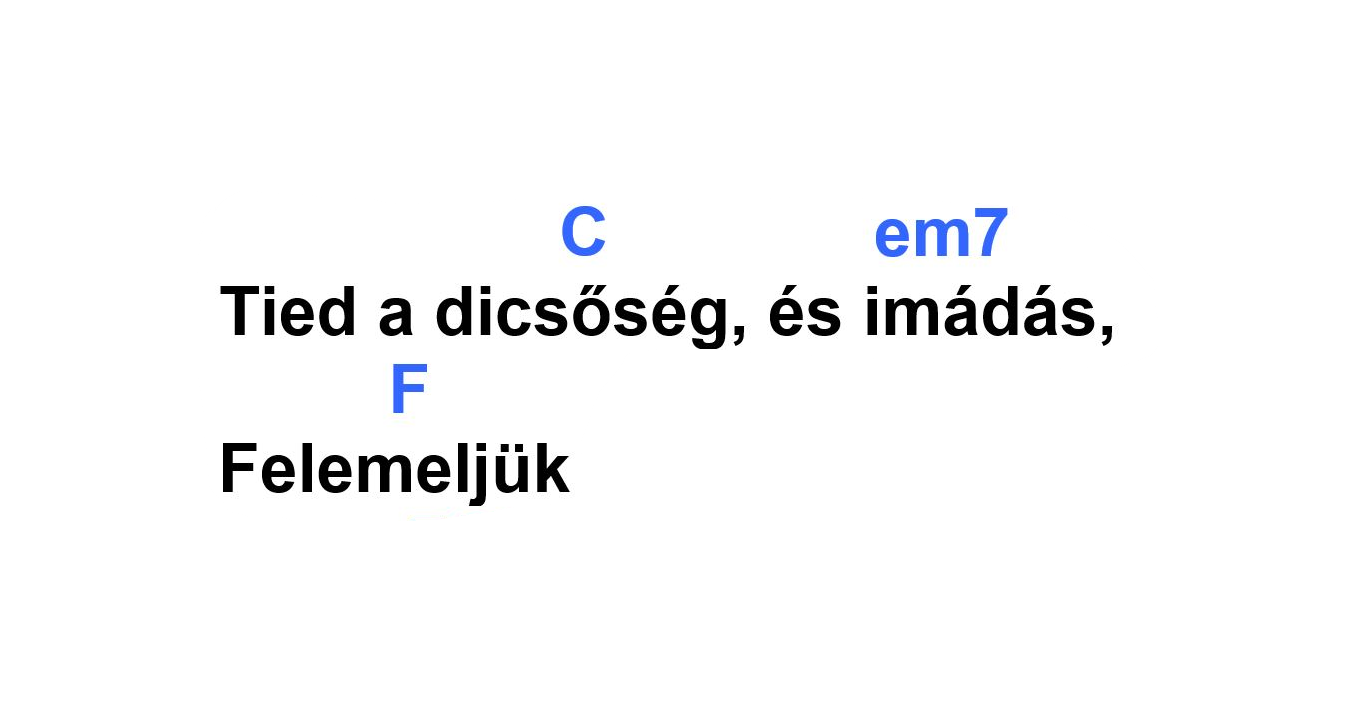
\includegraphics[scale=0.25]{images/representated_sheet.png}
	\caption{Az előző ábra végeredménye}
	\label{fig:repres2}
\end{figure}

\SubSection{Validáció}
A jelenlegi ábrázolás rendelkezik némi redundanciával. Ugye, ha azt tekintjük, hogy egy akkord három hanggal leírható, abban az esetben teljesen így lehet ábrázolni, de akkor kíván ez az adatszerkezet alidálást. Mi történik abban az esetben, ha az akkord három hangja, mondjuk mindegyik C hang. Ebben az esetben nem beszélhetünk akkordról, avagy hármas hangzatról, hiszen a hangköz távolság az nem megfelelő.
\par
Ehhez lenne szükség egy olyan fordítóra, ami az adatszerkezetet képes validálni. Itt viszont szükséges az, hogy a fordító ismerje az oktáv mind a tizenkettő hangját, ami alapján pontosan meg tudja határozni a hangközöket. A validálás egy olyan menetet követne, ahol az akkord, mint a 12-es szegmenst bemutató bővített xml struktúra a 3.3-as fejezetben, lenne vizsgálva, hogy megfelel e az akkrod típusnak azáltal, hogy a hangközök nagy - és kisterc távolságot követnek e.
\par
Emellett érdemes megfigyelni azt is, hogy a pozíció minden esetben csak a szegmenshez tartozó szövegből származhat. Így a fordító egy string visszakereséssel tudja majd leellenőrizni azt, hogy ez megvalósul e.
